\documentclass[11pt,a4paper]{article}

\usepackage[margin=1.5cm]{geometry}
\usepackage{graphicx}
\usepackage{amsmath}
\usepackage{listings}
\usepackage{xcolor}
\usepackage{hyperref}
\usepackage{tikz}
\usepackage{booktabs}
\usepackage{caption}

% Hyperlink configuration
\hypersetup{
    colorlinks=true,
    linkcolor=blue,
    filecolor=magenta,      
    urlcolor=blue,
    pdftitle={Computer Graphics Lab 4 Report},
    pdfauthor={Shahriar Alom Masud}
}

% Python syntax highlighting configuration
\definecolor{codegreen}{rgb}{0,0.55,0}
\definecolor{codegray}{rgb}{0.5,0.5,0.5}
\definecolor{codepurple}{rgb}{0.58,0,0.82}
\definecolor{backcolour}{rgb}{0.98,0.98,0.98}

\lstdefinestyle{pythonstyle}{
    backgroundcolor=\color{backcolour},   
    commentstyle=\color{codegreen}\itshape,
    keywordstyle=\color{blue}\bfseries,
    numberstyle=\tiny\color{codegray},
    stringstyle=\color{codepurple},
    basicstyle=\ttfamily\scriptsize,
    breaklines=true,                 
    numbers=left,                    
    numbersep=4pt,                  
    tabsize=4,
    frame=single,
    rulecolor=\color{lightgray}
}

\lstset{style=pythonstyle}

\begin{document}

% ==============================================================================
% COVER PAGE
% ==============================================================================
\begin{titlepage}
    % Page Border using TikZ
    \begin{tikzpicture}[remember picture, overlay]
        \draw[line width=1.2pt] 
            ([shift={(1.2cm,-1.2cm)}]current page.north west) 
            rectangle 
            ([shift={(-1.2cm,1.2cm)}]current page.south east);
        \draw[line width=0.5pt] 
            ([shift={(1.32cm,-1.32cm)}]current page.north west) 
            rectangle 
            ([shift={(-1.32cm,1.32cm)}]current page.south east);
    \end{tikzpicture}

    \centering
    \vspace*{0.4cm}

    % University Crest & Header
    
\includegraphics[width=3.6cm]{screenshots/uftb_logo.png}\\[0.4cm]
    {\normalsize \textbf{UNIVERSITY OF FRONTIER TECHNOLOGY, BANGLADESH}}\\[0.16cm]
    {\footnotesize \textbf{DEPARTMENT OF INTERNET OF THINGS AND ROBOTICS ENGINEERING (IRE)}}\\[0.14cm]
    {\footnotesize FACULTY OF CYBER PHYSICAL SYSTEM ENGINEERING}\\[0.55cm]

    % Divider Rule
    \noindent\rule{0.88\textwidth}{0.85pt}\\[0.85cm]

    % Header Title (Lab Topic)
    {\large \textbf{LAB REPORT 04}}\\[0.25cm]
    {\normalsize \textbf{3D WIREFRAME MODELING AND TRANSFORMATION USING OPENGL}}\\[0.85cm]

    % Course Code & Title
    {\normalsize \textbf{COURSE CODE: IRE 404}}\\[0.18cm]
    {\normalsize \textbf{COURSE TITLE: COMPUTER GRAPHICS AND ANIMATION SESSIONAL}}\\[1.0cm]

    % Student Info
    {\small \textbf{\underline{SUBMITTED BY:}}}\\[0.22cm]
    {\large \textbf{Shahriar Alom Masud}}\\[0.14cm]
    {\small Student ID: \textbf{2201032} \quad $\vert$ \quad Session: 2022--2023}\\[0.1cm]
    {\footnotesize Department of Internet of Things and Robotics Engineering (IRE), UFTB}\\[0.95cm]

    % Instructor Info
    {\small \textbf{\underline{SUBMITTED TO:}}}\\[0.22cm]
    {\large \textbf{Farzana Akter}}\\[0.14cm]
    {\small Assistant Professor}\\[0.1cm]
    {\footnotesize Department of Internet of Things and Robotics Engineering (IRE)}\\[0.08cm]
    {\footnotesize University of Frontier Technology, Bangladesh}

    % Date
    \vfill
    {\footnotesize NOVEMBER 16, 2026}
    \vspace*{0.3cm}
\end{titlepage}

\newpage
\pagenumbering{arabic}

% ==============================================================================
% 1. PROBLEM STATEMENT & OBJECTIVES
% ==============================================================================
\section*{1. Problem Statement and Objectives}
\noindent\rule{\textwidth}{0.6pt}\vspace{0.1cm}

The primary objective of this experiment is to construct, parameterize, and animate a 3D wireframe rectangular cuboid using the OpenGL state machine integrated within Pygame. While a cube has equal lengths along all axes ($X=Y=Z$), a rectangular cuboid requires mutually distinct dimensions ($W \neq H \neq D$), illustrating non-uniform spatial scaling and anisotropic perspective projection.

\vspace{0.15cm}
\noindent\textbf{Experimental Requirements:}
\begin{enumerate}
    \setlength{\itemsep}{0pt}
    \item Create an OpenGL rendering window with a resolution of $800 \times 600$ pixels via \texttt{pygame.display.set\_mode()}.
    \item Configure a solid black background color using \texttt{glClearColor(0.0, 0.0, 0.0, 1.0)}.
    \item Set the cuboid's wireframe edges to red using \texttt{glColor3f(1.0, 0.0, 0.0)}.
    \item Increase the stroke width of all edges to $3$ pixels using \texttt{glLineWidth(3.0)}.
    \item Modify standard cube coordinates to generate unequal width, height, and depth ($W=4.0, H=2.0, D=3.0$).
    \item Continuously rotate the cuboid around the $Y$-axis using \texttt{glRotatef(1.0, 0.0, 1.0, 0.0)}.
    \item Verify that the red rectangular cuboid rotates smoothly at 60 FPS against the solid black background.
\end{enumerate}

\noindent\textbf{GitHub Repository Link:}\\
\href{https://github.com/Masud744/Computer-Graphics-Lab/tree/main/Lab_04}{\texttt{https://github.com/Masud744/Computer-Graphics-Lab/tree/main/Lab\_04}}

% ==============================================================================
% 2. THEORETICAL & MATHEMATICAL FOUNDATION
% ==============================================================================
\vspace{0.25cm}
\section*{2. Theoretical and Mathematical Background}
\noindent\rule{\textwidth}{0.6pt}\vspace{0.1cm}

\subsection*{2.1 Geometric Modeling of Rectangular Cuboid}
A cuboid centered at the origin is characterized by half-extents $(w_x, h_y, d_z)$ such that $w_x \neq h_y \neq d_z$. We define:
$$\text{Width } (X) = 2 \times w_x = 4.0, \quad \text{Height } (Y) = 2 \times h_y = 2.0, \quad \text{Depth } (Z) = 2 \times d_z = 3.0$$
The 8 vertices $V_0, \dots, V_7$ are specified as $(\pm 2.0, \pm 1.0, \pm 1.5)$, interconnected by 12 boundary edges:
$$E = \{(0,1),(0,3),(0,4),(2,1),(2,3),(2,7),(6,3),(6,4),(6,7),(5,1),(5,4),(5,7)\}$$
Rendering is performed using the OpenGL primitive \texttt{GL\_LINES}.

\subsection*{2.2 Perspective Projection and Viewing Frustum}
Perspective projection produces realistic depth foreshortening wherein distant objects appear smaller. The projection matrix is generated via \texttt{gluPerspective($45^\circ, 800/600, 0.1, 50.0$)}. The scene is translated by $T(0, 0, -8.0)$ along the negative $Z$-axis to position the cuboid within the viewing frustum.

\subsection*{2.3 Continuous Rotation Matrix ($Y$-Axis)}
To animate continuous rotation around the Cartesian $Y$-axis, the transformation matrix $R_y(\theta)$ is applied each frame:
$$R_y(\theta) = \begin{bmatrix}
\cos\theta & 0 & \sin\theta & 0 \\
0 & 1 & 0 & 0 \\
-\sin\theta & 0 & \cos\theta & 0 \\
0 & 0 & 0 & 1
\end{bmatrix}$$
Calling \texttt{glRotatef(1.0, 0.0, 1.0, 0.0)} compounds this rotation into the current ModelView matrix at $60\text{ FPS}$, yielding smooth, constant-velocity angular displacement.

\newpage

% ==============================================================================
% 3. SOURCE CODE IMPLEMENTATION
% ==============================================================================
\section*{3. Python Source Code Implementation (\texttt{cuboid.py})}
\noindent\rule{\textwidth}{0.6pt}\vspace{0.15cm}

\lstinputlisting[language=Python]{../cuboid.py}

\newpage

% ==============================================================================
% 4. VISUALIZATION & OUTPUT
% ==============================================================================
\section*{4. Output Visualization and Verification}
\noindent\rule{\textwidth}{0.6pt}\vspace{0.06cm}

The program was executed on an $800 \times 600$ viewport. Below are four chronological captures illustrating the cuboid rotating smoothly around the $Y$-axis:

\vspace{0.08cm}
\begin{center}
    \begin{minipage}{0.38\textwidth}
        \centering
        
\includegraphics[width=\textwidth]{screenshots/cuboid_angle_0.png}
        \captionof{figure}{Initial orientation ($\theta = 0^\circ$)}
    \end{minipage}
    \hspace{0.5cm}
    \begin{minipage}{0.38\textwidth}
        \centering
        
\includegraphics[width=\textwidth]{screenshots/cuboid_angle_35.png}
        \captionof{figure}{Rotated state ($\theta = 35^\circ$)}
    \end{minipage}
    
    \vspace{0.08cm}
    \begin{minipage}{0.38\textwidth}
        \centering
        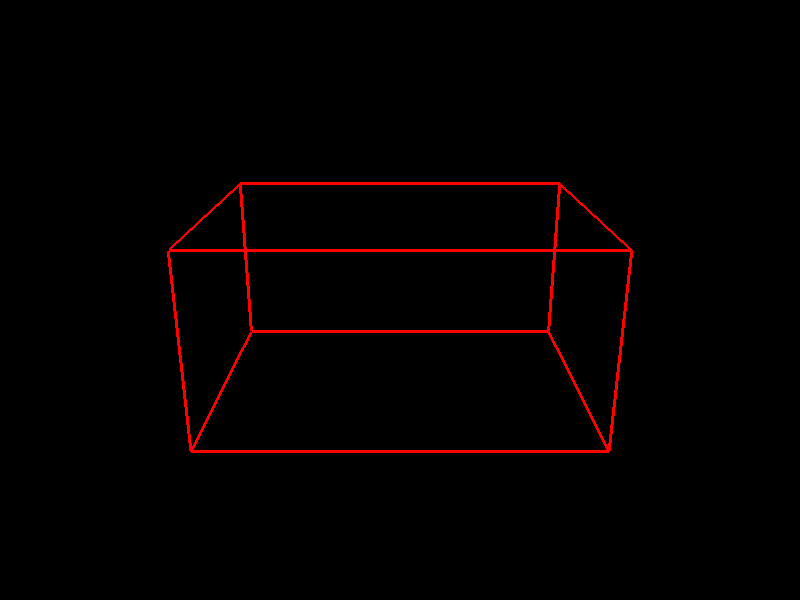
\includegraphics[width=\textwidth]{screenshots/cuboid_angle_70.png}
        \captionof{figure}{Rotated state ($\theta = 70^\circ$)}
    \end{minipage}
    \hspace{0.5cm}
    \begin{minipage}{0.38\textwidth}
        \centering
        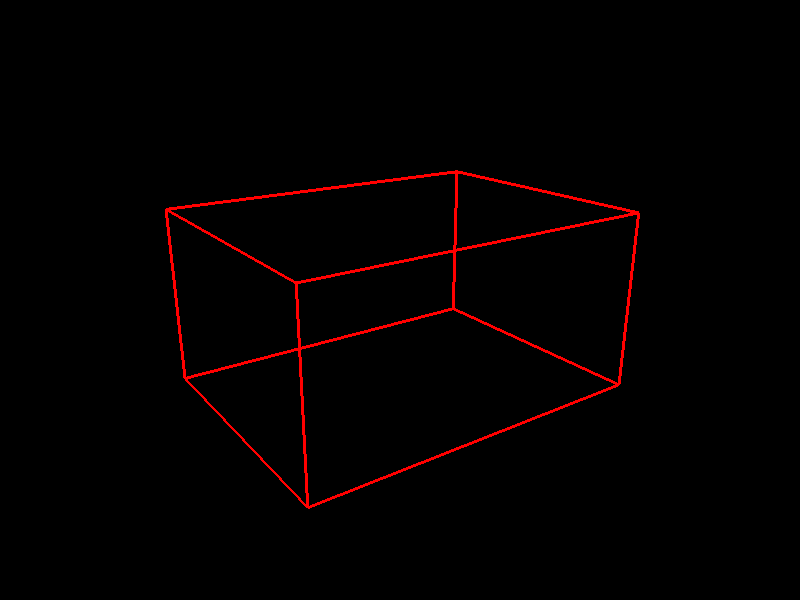
\includegraphics[width=\textwidth]{screenshots/cuboid_angle_120.png}
        \captionof{figure}{Rotated state ($\theta = 120^\circ$)}
    \end{minipage}
\end{center}

% ==============================================================================
% 5. REQUIREMENTS COMPLIANCE CHECKLIST
% ==============================================================================
\vspace{0.06cm}
\section*{5. Requirements Compliance Checklist}
\noindent\rule{\textwidth}{0.6pt}\vspace{0.04cm}

\begin{center}
\small
\begin{tabular}{cllc}
\toprule
\textbf{No.} & \textbf{Requirement Specification} & \textbf{Implementation in Source Code} & \textbf{Status} \\
\midrule
1 & $800 \times 600$ resolution window & \texttt{pygame.display.set\_mode((800, 600), DOUBLEBUF | OPENGL)} & \textbf{Verified} \\
2 & Black background color & \texttt{glClearColor(0.0, 0.0, 0.0, 1.0)} & \textbf{Verified} \\
3 & Red cuboid edges & \texttt{glColor3f(1.0, 0.0, 0.0)} inside \texttt{draw\_cuboid()} & \textbf{Verified} \\
4 & Edge line thickness $= 3$ px & \texttt{glLineWidth(3.0)} & \textbf{Verified} \\
5 & Unequal dimensions ($W \neq H \neq D$) & Width $= 4.0$, Height $= 2.0$, Depth $= 3.0$ & \textbf{Verified} \\
6 & Continuous $Y$-axis rotation & \texttt{glRotatef(1.0, 0.0, 1.0, 0.0)} inside render loop & \textbf{Verified} \\
7 & Smooth animation on black canvas & Hardware double-buffering at 60 FPS via \texttt{clock.tick(60)} & \textbf{Verified} \\
\bottomrule
\end{tabular}
\end{center}

% ==============================================================================
% 6. RESULTS & DISCUSSION
% ==============================================================================
\vspace{0.06cm}
\section*{6. Result and Discussion}
\noindent\rule{\textwidth}{0.6pt}\vspace{0.04cm}
{\small
The modified vertex coordinates accurately generated a rectangular cuboid rather than an equilateral cube. As the object undergoes continuous rotation around the vertical $Y$-axis, its unequal geometric proportions ($4.0 \times 2.0 \times 3.0$) are clearly visible through dynamic perspective foreshortening. The use of Pygame's \texttt{DOUBLEBUF} combined with \texttt{clock.tick(60)} ensures smooth, flicker-free rendering with crisp 3-pixel-wide red edges against the deep black background.
}

\end{document}
